% ============================================================
%  RL Course 2025/26 -- Group Project Report
%  Project spec: font 11pt, all margins 2.5 cm, line spacing 1.15
%  Max 15 pages (cover + appendices excluded)
% ============================================================
\documentclass[11pt,a4paper]{article}

\usepackage[utf8]{inputenc}
\usepackage[T1]{fontenc}
\usepackage{amsmath}
\usepackage{amssymb}
\usepackage{graphicx}
\usepackage{booktabs}
\usepackage{float}
\usepackage[margin=2.5cm]{geometry}
\usepackage[colorlinks=true, linkcolor=black, citecolor=black, urlcolor=black]{hyperref}

\linespread{1.15}

% Compact bullet lists
\let\olditemize\itemize
\renewcommand{\itemize}{%
  \olditemize
  \setlength{\itemsep}{1pt}
  \setlength{\topsep}{3pt}
  \setlength{\parsep}{0pt}
}

% NOVA IMS visual identity
\usepackage{helvet}
\renewcommand{\familydefault}{\sfdefault}
\usepackage{tikz}
\usetikzlibrary{calc}
\usepackage{fancyhdr}
\usepackage{xcolor}
\definecolor{imsdarkgrey}{RGB}{100,100,100}
\definecolor{imsmidgrey}{RGB}{175,175,175}
\definecolor{imslightgrey}{RGB}{240,240,240}
\definecolor{imsgreen}{RGB}{0,140,65}

% Placeholder helpers (remove before final submission)
% \todo{}         : short inline note
% \placeholder{}  : single-paragraph grey note (no environments inside)
% placeholderblock: multi-paragraph notes with lists/enumerates
\newcommand{\todo}[1]{\textbf{\textcolor{red}{[TODO: #1]}}}
\newcommand{\placeholder}[1]{\par\medskip\noindent{\small\color{gray}\textbf{[PLACEHOLDER]} #1}\par\medskip}
\newenvironment{placeholderblock}
  {\par\medskip\noindent\color{gray}\small\textbf{[PLACEHOLDER]}\par\noindent\rule{\linewidth}{0.3pt}\par}
  {\par\noindent\rule{\linewidth}{0.3pt}\par\medskip\normalcolor\normalsize}

\graphicspath{{../plots/}}

\begin{document}

% ── Cover page ───────────────────────────────────────────────
\thispagestyle{empty}
\begin{tikzpicture}[remember picture, overlay]
  \fill[imsgreen]
    ($(current page.north east)+(-2.97cm,0)$)
    rectangle (current page.south east);
  \begin{scope}
    \clip ($(current page.north east)+(-2.97cm,0)$)
          rectangle (current page.south east);
    \foreach \i in {0,1,...,130}{
      \draw[very thick,imsgreen!55!white]
        ($(current page.north east)+(0,-\i*2.8mm)$) -- ++(-3.5cm,3.5cm);
    }
  \end{scope}
  \fill[imsgreen]
    (current page.north west)
    rectangle ($(current page.north east)+(0,-12pt)$);
  \fill[imslightgrey]
    (current page.south west)
    rectangle ($(current page.south east)+(-2.97cm,1.2cm)$);
\end{tikzpicture}

\vspace*{1.8cm}
\begin{minipage}[t]{\dimexpr\textwidth-0.8cm\relax}
  \sffamily\color{imsdarkgrey}
  {\small\bfseries NOVA Information Management School}\\[0.2em]
  {\small Master in Data Science and Advanced Analytics}\\[0.1em]
  {\small Data Science Specialisation}

  \vspace{2.5cm}

  {\LARGE\bfseries Reinforcement Learning for Sepsis\\[0.3em]
  Treatment Optimisation}

  \vspace{1.5cm}

  {\small\bfseries Course}\\[0.2em]
  {\small Reinforcement Learning}\\[0.3em]
  {\small Academic Year 2025/26}

  \vspace{0.6cm}

  {\small\bfseries Group Members}\\[0.3em]
  {\small Moritz Baldauf -- 20250370}\\[0.2em]
  {\small Ozougwu Chukwuebuka -- 20250449}\\[0.2em]
  {\small Miguel Oliveira -- 20250379}\\[0.2em]
  {\small Simon Sazonov -- 20221689}

\end{minipage}

\newpage

% ── Body page style ──────────────────────────────────────────
\pagestyle{fancy}
\fancyhf{}
\renewcommand{\headrulewidth}{1pt}
\renewcommand{\headrule}{%
  \begingroup\color{imsgreen}%
  \hrule height \headrulewidth width \headwidth%
  \endgroup}
\renewcommand{\footrulewidth}{0pt}
\fancyhead[L]{\sffamily\footnotesize\color{imsdarkgrey} Reinforcement Learning 2025/26}
\fancyhead[R]{\sffamily\footnotesize\color{imsdarkgrey}\nouppercase{\leftmark}}
\fancyfoot[C]{\sffamily\small\color{imsdarkgrey}\thepage}
\renewcommand{\sectionmark}[1]{\markboth{#1}{}}

\tableofcontents
\newpage

% ============================================================
\section{Introduction}
\label{sec:intro}
% ============================================================

Sepsis is a life-threatening syndrome in which the body's dysregulated immune
response to infection causes progressive organ dysfunction. With an estimated
49 million incident cases and 11 million attributable deaths globally in
2017~\cite{rudd2020}, it ranks among the most common causes of intensive care
unit (ICU) mortality. The clinical definition was formalised by the Sepsis-3
consensus~\cite{singer2016}, which emphasises the heterogeneity of patient
presentations and the absence of a single universal treatment protocol.

The two principal pharmacological interventions are vasopressor administration,
which maintains systemic blood pressure by inducing vasoconstriction, and
intravenous (IV) fluid resuscitation, which sustains circulatory volume.
Both must be titrated continuously against the patient's evolving state:
insufficient dosing risks life-threatening hypotension (low blood pressure) while
excessive loading causes pulmonary oedema (fluid overload in the lungs) and
secondary organ failure. Outcomes are observable
only at episode end, making credit assignment across the treatment trajectory
the central algorithmic challenge.

This decision structure maps naturally onto a sequential MDP: the agent observes
a snapshot of patient physiology at each step, selects a joint (vasopressor,
IV fluid) action, and receives a delayed binary reward -- survival or death --
reflecting the cumulative effect of all prior decisions.
Komorowski et al.~\cite{komorowski2018} demonstrated on the MIMIC-III clinical
database that an RL-derived policy achieved lower 90-day mortality than
clinician-administered treatments, establishing the clinical feasibility of the
approach and the data foundation for the ICU-Sepsis-v2 benchmark used here.

ICU-Sepsis-v2 formalises this as an episodic MDP with a sparse terminal reward
($+1$ survival, $0$ death) and 25 discrete (vasopressor, IV fluid) actions.
Two configurations of increasing observational complexity were provided:

\begin{itemize}
  \item \textbf{Config A (discrete):} integer state index (0--715) encoding the
        patient's clinical presentation, with the full transition matrix $P$ and
        reward matrix $R$ accessible.
  \item \textbf{Config B (continuous):} 47-dimensional physiological feature
        vector~\cite{komorowski2018} with three clinical reality wrappers adding
        observation noise (prob.\,0.15), randomly missing features (prob.\,0.15),
        and acute deterioration events (prob.\,0.01 per step).
\end{itemize}

The environment, configurations, and evaluation functions were provided as
course infrastructure; algorithm implementations, hyperparameter tuning, and
extensions are the original contribution of this work. Three extensions are
developed beyond the two required algorithms per configuration: SOFA-delta
reward shaping to address the sparse credit-assignment problem, a failure-mode
ablation isolating each Config B wrapper's independent impact, and a Pareto
frontier analysis mapping the survival--intensity trade-off across $\lambda$.


% ============================================================
\section{Methodology}
\label{sec:methodology}
% ============================================================

% ── 2.1 ─────────────────────────────────────────────────────
\subsection{Configuration A: Tabular Methods}
\label{sec:method_a}
% ─────────────────────────────────────────────────────────────

Config A presents a discrete MDP with 716 states and 25 actions whose Q-table
requires only 17\,900 entries. Although the full transition matrix $P$ and reward
matrix $R$ are both provided, enabling model-based approaches such as policy
iteration, three model-free temporal-difference (TD) algorithms were selected.
We chose model-free algorithms to build up the foundation of our analysis and avoid 
beeing districtated by artificially good results of model-based approaches, that are 
not possible to be replicated in a real world setting. 
The discrete, fully enumerable state space makes Config A a controlled setting
in which the on-policy versus off-policy distinction and the effect of
overestimation bias can be cleanly isolated, without the confounding influence
of function approximation error introduced in Config B.

\paragraph{Q-Learning.}
Q-Learning is an off-policy TD algorithm that learns the optimal action-value
function $Q^*(s, a)$ by bootstrapping from the greedy maximum over next-state
values:
\begin{equation}
  Q(s, a) \;\leftarrow\; Q(s, a)
    + \alpha\bigl[r + \gamma \max_{a'} Q(s', a') - Q(s, a)\bigr].
  \label{eq:ql}
\end{equation}
The target always uses the greedy maximum regardless of which action the
$\varepsilon$-greedy behaviour policy actually selected, making the algorithm
off-policy by construction. Q-Learning was chosen as the natural off-policy
baseline: it is the most direct algorithmic expression of the Bellman optimality
operator on a finite Q-table.

\paragraph{SARSA.}
SARSA is an on-policy TD algorithm that replaces the greedy maximum in
Equation~\ref{eq:ql} with the value of the action actually drawn from the
current $\varepsilon$-greedy policy:
\begin{equation}
  Q(s, a) \;\leftarrow\; Q(s, a)
    + \alpha\bigl[r + \gamma Q(s', a') - Q(s, a)\bigr],
  \label{eq:sarsa}
\end{equation}
where $a' \sim \pi_\varepsilon(\cdot \mid s')$. Because the update target
reflects the policy actually followed, SARSA penalises state-action pairs
that lead to exploratory, potentially suboptimal transitions rather than
assuming perfect future greedy behaviour. This conservative property is
directly relevant to the clinical setting, where the cost of overestimating
the value of a state that precedes a random exploratory action is a
misjudged treatment recommendation.

\paragraph{Double Q-Learning.}
Standard Q-Learning suffers from overestimation bias: the $\max$ operator in
Equation~\ref{eq:ql} systematically selects the action with the highest noise
in $Q$ rather than the highest true value, and the inflated estimates compound
over successive updates. Double Q-Learning~\cite{hasselt2010} addresses this by
maintaining two Q-tables updated alternately at random. On each step one table
selects the greedy action; the other evaluates it:
\begin{equation}
  a^* = \arg\max_{a'} Q_1(s', a'), \quad
  \text{target} = r + \gamma Q_2(s', a^*),
  \label{eq:dql}
\end{equation}
and symmetrically with $Q_1$ and $Q_2$ swapped. Decoupling selection from
evaluation eliminates the positive correlation that drives overestimation in
standard Q-Learning. Double Q-Learning was included to test whether this
bias-correction improves performance in the sparse-reward, 716-state Config A
MDP, or whether the added variance from maintaining two independent tables
outweighs the benefit.

\paragraph{Shared settings.}
All three algorithms use $\gamma = 1.0$ (undiscounted), appropriate for a
task in which the only reward signal is a terminal binary outcome.
Exploration follows an $\varepsilon$-greedy schedule from
$\varepsilon_{\text{start}} = 1.0$ to $\varepsilon_{\text{end}} = 0.05$.
Starting at full exploration ensures every state in the 716-state space is
visited before the policy commits to a greedy direction; the floor of $0.05$
retains a small residual exploration rate at convergence to prevent the policy
from fixating on a locally visited region of the MDP.

\paragraph{Hyperparameter tuning.}
The learning rate $\alpha$ and $\varepsilon$-decay schedule jointly govern the
speed and stability of Q-value convergence: too large an $\alpha$ causes
oscillating updates in a sparse-reward MDP where individual transitions carry
high signal variance, while too slow a decay schedule prolongs the exploration
phase at the expense of exploitation. Tuning each algorithm to its best
configuration is necessary for a fair cross-algorithm comparison: comparing
algorithms at their respective defaults would conflate hyperparameter
sensitivity with fundamental algorithmic differences, obscuring the actual
on-policy versus off-policy trade-off under study.

A grid search was therefore conducted over $\alpha \in \{0.05, 0.1, 0.3, 0.5\}$
and $\varepsilon$-decay schedule $\in \{\text{linear, exponential, GLIE}\}$,
yielding 12 candidate configurations for Q-Learning and SARSA. For Double
Q-Learning the decay was fixed to linear and only $\alpha$ was swept, giving
4 candidates. Each candidate was trained for 20\,000 episodes and evaluated on
50 greedy rollouts on a held-out validation set; the configuration maximising
validation survival rate was selected. Final models were then trained for
50\,000 episodes under the selected hyperparameters. The selected
configurations are summarised in Table~\ref{tab:hparam_a}.

\begin{table}[H]
\centering\small
\caption{Selected hyperparameters for Config A algorithms.
         Common settings: $\gamma=1.0$, $\varepsilon_{\text{start}}=1.0$,
         $\varepsilon_{\text{end}}=0.05$, 50\,000 training episodes.}
\label{tab:hparam_a}
\begin{tabular}{lcc}
\toprule
Algorithm & $\alpha$ & $\varepsilon$-decay \\
\midrule
Q-Learning        & 0.1 & GLIE \\
SARSA             & 0.3 & Exponential \\
Double Q-Learning & 0.1 & Linear (fixed) \\
\bottomrule
\end{tabular}
\end{table}

% ── 2.2 ─────────────────────────────────────────────────────
\subsection{Configuration B: Function Approximation}
\label{sec:method_b}
% ─────────────────────────────────────────────────────────────

Config B replaces the discrete state with a 47-dimensional continuous
physiological feature vector, making the Q-table infinite-dimensional and
tabular methods fundamentally inapplicable. Three clinical reality wrappers
further increase environment difficulty: an observation noise wrapper that
corrupts sensor readings with probability 0.15, a missing-observation wrapper
that randomly masks up to 4 features per step with probability 0.15, and an
acute-event wrapper that introduces sudden patient deteriorations with
probability 0.01 per step. Together these wrappers introduce irreducible
stochasticity that no memorised lookup policy can compensate for, requiring
algorithms that generalise across unseen feature combinations.

Three algorithms spanning the spectrum from linear to deep function
approximation were selected: a linear baseline that bridges directly from the
tabular approach, an off-policy deep RL method, and an on-policy deep RL
method. This design allows the non-linear capacity of neural networks and the
on-policy versus off-policy distinction to be evaluated independently under
identical step budgets.

\paragraph{Linear SARSA-FA.}
Linear function approximation represents the action-value function as a linear
combination of the input features for each action:
\begin{equation}
  Q(s, a;\, W) = W_a^\top \phi(s),
  \label{eq:lfa}
\end{equation}
where $W$ is a $(25 \times 47)$ weight matrix and $\phi(s)$ is the normalised
47-dimensional feature vector. Weights are updated via the on-policy SARSA
TD(0) rule:
\begin{equation}
  \delta = r + \gamma\, Q(s', a';\, W) - Q(s, a;\, W), \qquad
  W_a \;\leftarrow\; W_a + \alpha\,\delta\,\phi(s).
  \label{eq:lfa_update}
\end{equation}
A single weight update generalises immediately to all states that share similar
feature vectors, which is essential when the continuous observation space makes
full state coverage impossible. Linear SARSA-FA was chosen as a deliberate
bridge method: it preserves the on-policy SARSA update from Config A while
introducing the minimum architectural change required for continuous states.
If it matches DQN performance, the non-linear capacity of neural networks is
unnecessary at this step budget.

\paragraph{Deep Q-Network (DQN).}
DQN replaces the linear weight matrix with a neural network
$Q(s, a;\, \theta)$ mapping the 47-dimensional observation to Q-values for
all 25 actions simultaneously. The network architecture is:
\[
  47 \rightarrow 64\text{ (ReLU)} \rightarrow 64\text{ (ReLU)} \rightarrow 25.
\]
Two stabilising techniques distinguish DQN from naive deep Q-Learning.
\textit{Experience replay} stores transitions $(s, a, r, s')$ in a replay
buffer and samples uniformly at each update step, breaking the temporal
correlations between consecutive transitions that would otherwise destabilise
gradient descent. \textit{Target network}: a frozen copy of the Q-network,
synchronised every \texttt{target\_update\_interval} steps, provides stable
regression targets and prevents the moving-target problem in which both the
prediction and the target shift simultaneously. DQN was selected as the
natural off-policy deep RL baseline, directly extending Q-Learning to the
continuous state space.

\paragraph{Proximal Policy Optimization (PPO).}
PPO is an on-policy actor-critic algorithm that directly optimises a
stochastic policy $\pi(a \mid s;\, \theta)$ using the clipped surrogate
objective:
\begin{equation}
  L_{\text{CLIP}}(\theta) = \mathbb{E}\!\left[\min\!\left(
      r_t(\theta)\,A_t,\;
      \text{clip}\!\bigl(r_t(\theta),\,1{-}\varepsilon_c,\,1{+}\varepsilon_c\bigr)
      A_t\right)\right],
  \label{eq:ppo}
\end{equation}
where $r_t(\theta) = \pi(a_t \mid s_t;\,\theta)\,/\,\pi_{\text{old}}(a_t \mid s_t)$
is the probability ratio and $A_t$ the generalised advantage estimate. The clip
bounds the ratio to $[1{-}\varepsilon_c,\, 1{+}\varepsilon_c]$, preventing
destructively large policy updates. PPO collects $n_{\text{steps}}$ on-policy
rollouts before each gradient update and applies $n_{\text{epochs}}$ passes
over the collected batch. An entropy bonus (coefficient \texttt{ent\_coef})
discourages premature policy collapse. PPO was chosen to represent the on-policy
deep RL family: comparing it to DQN under the same step budget isolates the
effect of on-policy versus off-policy learning in this partially-observable,
sparse-reward environment.

\paragraph{Shared settings.}
All Config B algorithms use $\gamma = 1.0$ consistent with Config A. DQN and PPO
were implemented via \texttt{stable-baselines3} with a \texttt{LearningCurveCallback}
that periodically evaluates the greedy policy on a held-out validation set and
saves the best checkpoint, ensuring the returned model is the highest-performing
snapshot rather than the final iterate. The training budget was fixed at 100\,000
steps for both DQN and PPO to ensure a fair comparison; Linear SARSA-FA used
a budget of 20\,000 episodes, selected by grid search.

\paragraph{Hyperparameter tuning.}
A two-phase protocol was applied to DQN and PPO. Phase one ran a coarse grid
search over learning rate at 30\,000 steps; phase two used Optuna
TPE~\cite{akiba2019} to search jointly over the remaining hyperparameters for
15 trials, with the phase-one LR as anchor, and retrained the best
configuration for the full 100\,000-step budget. For Linear SARSA-FA, a full
grid over $\alpha$ and episode budget was feasible given the low per-episode
cost. Selected hyperparameters are in Table~\ref{tab:hparam_b}.

\begin{table}[H]
\centering\small
\caption{Selected hyperparameters for Config B algorithms.
         Common: $\gamma=1.0$, $\varepsilon_{\text{start}}=1.0$,
         $\varepsilon_{\text{end}}=0.05$.}
\label{tab:hparam_b}
\begin{tabular}{llr}
\toprule
Algorithm & Hyperparameter & Selected value \\
\midrule
Linear SARSA-FA & Learning rate $\alpha$          & $0.001$ \\
                & Training episodes               & $20\,000$ \\
\midrule
DQN             & Learning rate                   & $3.72 \times 10^{-4}$ \\
                & Target update interval (steps)  & $1\,000$ \\
                & Replay buffer size              & $20\,000$ \\
\midrule
PPO             & Learning rate                   & $1.73 \times 10^{-4}$ \\
                & Rollout steps $n_{\text{steps}}$& $1\,024$ \\
                & Clip range $\varepsilon_c$      & $0.77$ \\
                & Entropy coefficient             & $7.8 \times 10^{-4}$ \\
\bottomrule
\end{tabular}
\end{table}


% ============================================================
\section{Evaluation and Comparative Analysis}
\label{sec:evaluation}
% ============================================================

% ── 3.1 ─────────────────────────────────────────────────────
\subsection{Configuration A Results}
\label{sec:eval_a}
% ─────────────────────────────────────────────────────────────

All three algorithms were evaluated on a held-out test set of 200 episodes
with a fixed seed, against a random baseline estimated over 1\,000 episodes.
Test survival rates and mean returns are reported in Table~\ref{tab:results_a}.

\begin{table}[H]
\centering\small
\caption{Config A test results (200 episodes, fixed seed; random baseline over
         1\,000 episodes). Survival 95\,\% CIs computed via the Wilson interval.
         Mean return is lower than survival rate due to the $\lambda=0.02$
         treatment intensity penalty.}
\label{tab:results_a}
\begin{tabular}{lcccc}
\toprule
Algorithm & Survival\,\% & 95\,\% CI & Mean return & Intensity tax \\
\midrule
Random baseline   & 68.5 & [65.6, 71.3] & 0.605 & 0.102 \\
Q-Learning        & 69.0 & [62.3, 75.0] & 0.609 & 0.081 \\
SARSA             & 70.0 & [63.3, 75.9] & 0.617 & 0.083 \\
Double Q-Learning & 67.5 & [60.7, 73.6] & 0.608 & 0.067 \\
\bottomrule
\end{tabular}
\end{table}

SARSA ($70.0\,\%$) outperforms Q-Learning ($69.0\,\%$) by $1.0$\,pp, and
Q-Learning outperforms Double Q-Learning ($67.5\,\%$) by $1.5$\,pp. The
most striking result is that Double Q-Learning falls $1.0$\,pp \emph{below}
the random baseline, despite being the theoretically most sophisticated of
the three algorithms.

The SARSA advantage is consistent with its on-policy update structure: by
optimising the policy it actually follows rather than a hypothetical greedy
policy, SARSA accumulates more stable Q-estimates in this sparse-reward MDP.
Q-Learning's off-policy max-bootstrap introduces overestimation bias (shown
in Figure~\ref{fig:config_a_overestimation}) that inflates Q-values, which
can misdirect the greedy policy toward states that appear high-value but are
not. The gap between SARSA and Q-Learning ($1.9$\,pp in training survival,
$1.0$\,pp in test survival) reflects this trade-off between on-policy safety
and off-policy efficiency.

Double Q-Learning's underperformance below the random baseline is the most
counterintuitive result. Bias correction is only beneficial if the
overestimation is large enough to cause policy errors that outweigh the cost
of the doubled variance. In a 716-state MDP with 97.9\,\% Q-table coverage
and 50\,000 training episodes, overestimation bias is relatively mild because
the agent has visited most state-action pairs many times. The halved effective
update rate introduced by the two-table alternation then costs more in
convergence speed than the bias correction recovers, leaving the final policy
marginally worse than random.

\subsubsection{Learning dynamics}
Figure~\ref{fig:config_a_learning} shows two complementary views of the
training process. The left panel plots the 500-episode smoothed training
return for all three algorithms; the right panel shows the greedy survival
rate measured every 2\,000 episodes by evaluating the current policy with
$\varepsilon=0$ on 50 fixed rollouts, removing all exploration noise from
the measurement.

Both panels confirm that learning occurred. The training curves rise from
near the random baseline during the high-$\varepsilon$ exploration phase
(episodes 0--5\,000) and climb steadily as $\varepsilon$ decays and TD
updates propagate the sparse survival signal backward through visited
state-action pairs. The greedy evaluation curves provide the cleaner signal:
each algorithm's $\varepsilon=0$ policy improves monotonically over training
checkpoints, establishing that the Q-tables are genuinely accumulating
knowledge rather than improving through reduced exploration noise alone.
Convergence is exploration-decay-limited rather than sample-limited: extending
the budget beyond 50\,000 episodes would yield diminishing returns. Double
Q-Learning converges more slowly because each transition updates only one
table at random, halving the effective update frequency.

\begin{figure}[H]
  \centering
  \begin{minipage}[t]{0.49\textwidth}
    \centering
    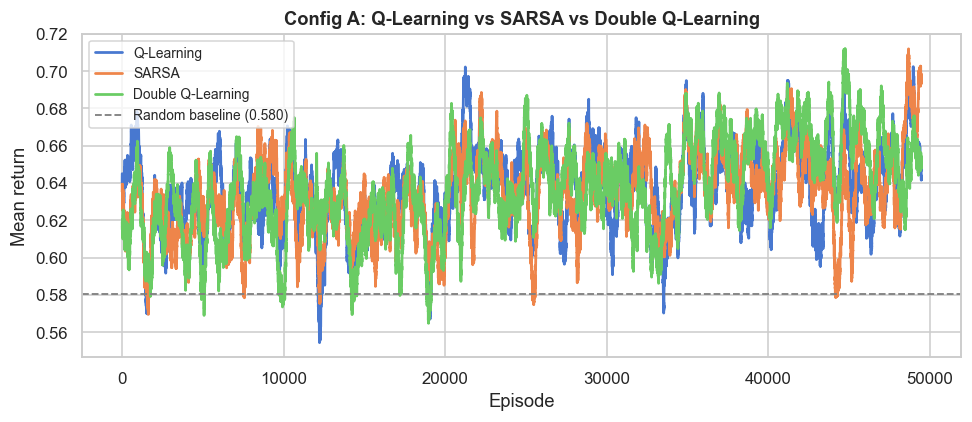
\includegraphics[width=\linewidth, height=5cm]{configA_triple_curves.png}
  \end{minipage}
  \hfill
  \begin{minipage}[t]{0.49\textwidth}
    \centering
    \includegraphics[width=\linewidth, height=5cm]{configA_greedy_eval.png}
  \end{minipage}
  \caption{Config A learning dynamics. \textit{Left}: smoothed training
  returns (500-episode window). \textit{Right}: greedy policy survival rate
  evaluated every 2\,000 episodes at $\varepsilon=0$, isolating policy
  quality from exploration noise. All three algorithms improve monotonically;
  convergence plateaus at episode $\approx$35\,000--40\,000 when
  $\varepsilon$ reaches its floor.}
  \label{fig:config_a_learning}
\end{figure}


\paragraph{Overestimation bias}
Q-Learning consistently overestimates state values above $V^*$ (computed
exactly via value iteration on the provided MDP matrices), particularly in
states with high survival probability where the max-bootstrap target amplifies
positive noise. Double Q-Learning's decoupled estimation visibly reduces this
gap, confirming the bias-correction mechanism is active, yet the test survival
outcome is still worse, isolating the added variance as the proximate cause of
underperformance (see Appendix~\ref{app:overestimation}).

\paragraph{Policy interpretation}
The learned SARSA policy is analysed alongside the Config B weight matrix in
Section~\ref{sec:eval_cross}, where a direct cross-configuration comparison
of agent behaviour is presented.

% ── 3.2 ─────────────────────────────────────────────────────
\subsection{Configuration B Results}
\label{sec:eval_b}
% ─────────────────────────────────────────────────────────────

All three Config B algorithms were evaluated on the same held-out test set
as Config A (200 episodes, fixed seed). Test results are reported in
Table~\ref{tab:results_b}.

\begin{table}[H]
\centering\small
\caption{Config B test results (200 episodes, fixed seed; random baseline over
         1\,000 episodes). Survival 95\,\% CIs via Wilson interval. Mean return
         is lower than survival rate due to the $\lambda=0.02$ intensity penalty.}
\label{tab:results_b}
\begin{tabular}{lcccc}
\toprule
Algorithm & Survival\,\% & 95\,\% CI & Mean return & Intensity tax \\
\midrule
Random baseline (clinical) & 67.0 & [63.9, 69.7] & 0.579 & 0.090 \\
Linear SARSA-FA            & 61.5 & [54.7, 67.9] & 0.568 & 0.027 \\
DQN                        & 61.5 & [54.7, 67.9] & 0.487 & 0.078 \\
PPO                        & 60.5 & [53.7, 67.3] & 0.538 & 0.087 \\
\bottomrule
\end{tabular}
\end{table}

Linear SARSA-FA and DQN tie at $61.5\,\%$, with PPO $1.0$\,pp behind at
$60.5\,\%$. The tie is the central finding of Config B: at a budget of
100\,000 steps, the non-linear representational capacity of a
two-hidden-layer network provides no measurable advantage over a linear
weight matrix. As visible in Figure~\ref{fig:config_b_algorithms}, Linear
SARSA-FA arrives at the same endpoint at a fraction of the computational
cost; DQN's harder optimisation landscape, compounded by the replay buffer
warm-up period, fully offsets the expressive power gained.

PPO's marginal underperformance relative to DQN is consistent with the
on-policy disadvantage in sparse-reward settings: the stochastic policy
distributes probability mass over suboptimal actions, producing slightly
worse expected treatment decisions than DQN's deterministic greedy policy.
The low optimal entropy coefficient ($7.8 \times 10^{-4}$, selected by
Optuna) confirms this: once the policy begins concentrating on high-survival
actions, additional entropy regularisation actively reduces performance.

\subsubsection{Learning dynamics}
Figure~\ref{fig:config_b_algorithms} shows training curves for all three
algorithms; none crosses the $67.0\,\%$ random baseline, though this
reflects environmental difficulty rather than a failure to learn. Greedy
evaluation curves separating policy improvement from exploration noise are
in Appendix~\ref{app:greedy_eval}: DQN gains ${\approx}11.5$\,pp from
initialisation to convergence, confirming genuine learning despite ending
below the baseline.

\begin{figure}[H]
  \centering
  \begin{minipage}[t]{0.49\textwidth}
    \centering
    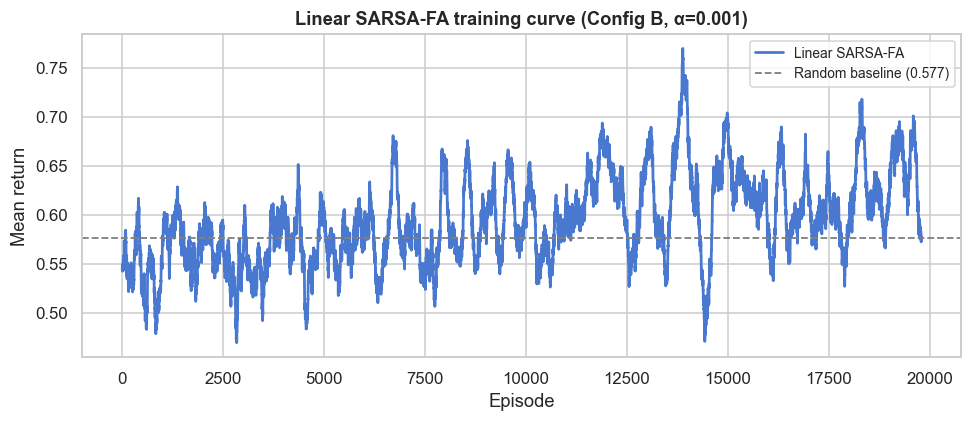
\includegraphics[width=\linewidth, height=5cm]{configB_lfa_curve.png}
  \end{minipage}
  \hfill
  \begin{minipage}[t]{0.49\textwidth}
    \centering
    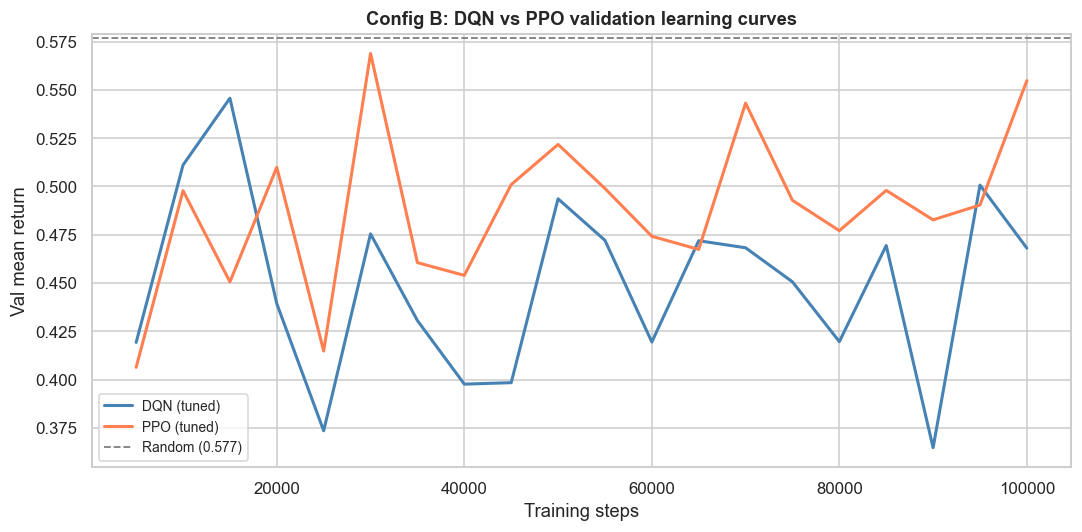
\includegraphics[width=\linewidth, height=5cm]{configB_dqn_ppo_curves.png}
  \end{minipage}
  \caption{Config B training curves. \textit{Left}: Linear SARSA-FA training
  return (smoothed) versus the random baseline; the curve flattens around
  15\,000 episodes. \textit{Right}: DQN and PPO tuned validation curves;
  both plateau around 60\,000--70\,000 steps as the sparse reward exhausts
  the gradient signal. None of the three algorithms crosses the $67.0\,\%$
  random baseline.}
  \label{fig:config_b_algorithms}
\end{figure}

\subsubsection{Hyperparameter tuning impact}
Both DQN and PPO tuned configurations outperform their defaults by
approximately $1$--$2$\,pp in validation survival (Appendix~\ref{app:tuning}).
The gain is modest because the binding constraint is the sparse reward signal
rather than suboptimal hyperparameters: even with optimal parameters, the
100\,000-step budget provides limited gradient information per episode in a
task with binary terminal rewards
(Optuna importance plots in Appendix~\ref{app:optuna}).

% ── 3.3 ─────────────────────────────────────────────────────
\subsection{Cross-Configuration Comparison}
\label{sec:eval_cross}
% ─────────────────────────────────────────────────────────────

Figure~\ref{fig:crossconfig} places all eight results (six algorithms and
two random baselines) on a single axis. The best Config A agent (SARSA,
$70.0\,\%$) outperforms the best Config B agent (Linear SARSA-FA / DQN,
$61.5\,\%$) by $8.5$\,pp.

\begin{figure}[H]
  \centering
  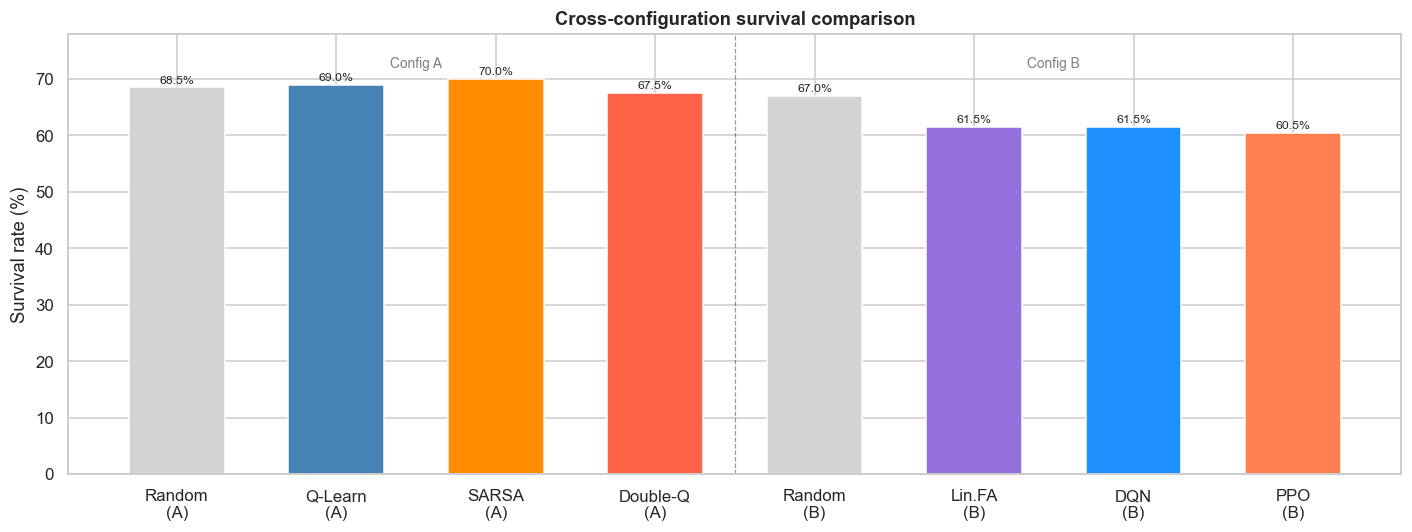
\includegraphics[width=\textwidth]{crossconfig_survival.png}
  \caption{Test survival rates for all six algorithms and both random
  baselines. Config A algorithms (left group) cluster near or above their
  $68.5\,\%$ random baseline; Config B algorithms (right group) all fall
  below their $67.0\,\%$ baseline. The $8.5$\,pp gap between the best
  Config A and Config B results is attributable to two compounding factors
  described in the text.}
  \label{fig:crossconfig}
\end{figure}

Two compounding factors drive the $8.5$\,pp gap. First, the three clinical
reality wrappers in Config B inject irreducible stochasticity: acute events
alone account for $5.4$\,pp of survival degradation (quantified in
Section~\ref{sec:ablation}), a loss that no policy can recover regardless
of its representational capacity, because sudden patient deterioration
terminates the episode independently of the treatment administered. Second,
the continuous state space requires generalisation across never-before-seen
feature combinations rather than memorising state-specific values; even with
$97.9\,\%$ Q-table coverage in Config A, the tabular agent can exploit exact
transition probabilities that are unavailable in Config B.

\paragraph{Policy behaviour across configurations}
Figure~\ref{fig:policy_comparison} contrasts agent behaviour across the two
configurations. In Config A, the SARSA policy is directly observable as a
$5{\times}5$ action-distribution heatmap: most of the 714 non-terminal states
map to low-vasopressor, low-to-medium fluid actions, with high-vasopressor
actions reserved for a small subset corresponding to severe presentations.
The agent learned a state-dependent, clinically coherent treatment strategy
rather than collapsing to a degenerate fixed action.

In Config B, the continuous state space makes the policy unobservable in the
same way. The Linear SARSA-FA weight matrix serves as a proxy for feature
importance. This shift -- from directly inspecting action distributions to
inspecting feature weights -- illustrates why interpretability becomes harder
as observation complexity grows.

\begin{figure}[H]
  \centering
  \begin{minipage}[t]{0.49\textwidth}
    \centering
    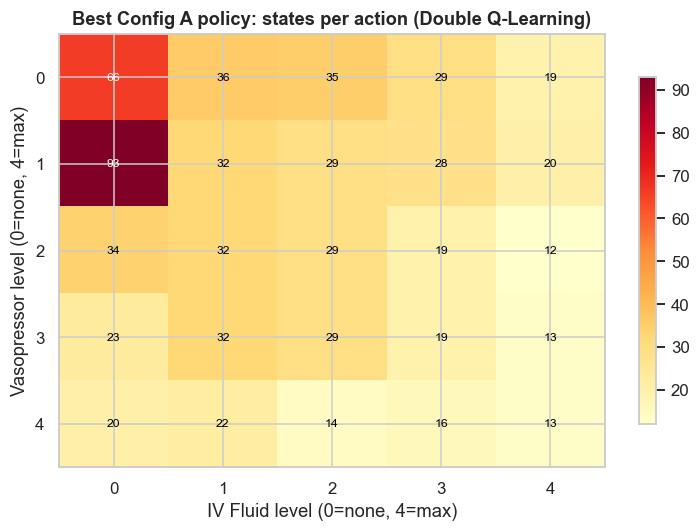
\includegraphics[width=\linewidth, height=5.5cm]{configA_policy_heatmap.png}
  \end{minipage}
  \hfill
  \begin{minipage}[t]{0.49\textwidth}
    \centering
    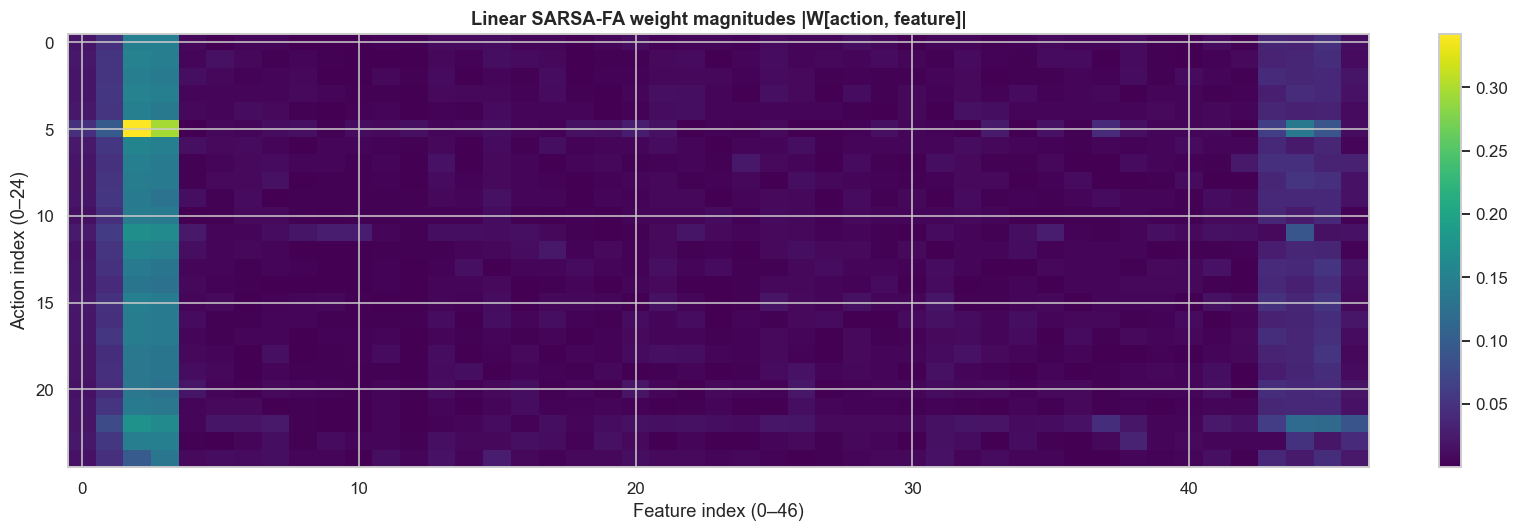
\includegraphics[width=\linewidth, height=5.5cm]{configB_lfa_weights.png}
  \end{minipage}
  \caption{Policy behaviour across configurations. \textit{Left}: SARSA
  action-distribution heatmap (Config A) -- each cell counts the number of
  non-terminal states ($n=714$) for which that (vasopressor, IV fluid) pair
  is greedy, showing a conservative, clinically coherent profile.
  \textit{Right}: Linear SARSA-FA weight magnitude heatmap (Config B) --
  each cell shows $|W_{a,f}|$ for action $a$ and feature $f$; sparse
  high-magnitude entries confirm the agent relies on a small subset of
  physiologically meaningful features rather than fitting noise.}
  \label{fig:policy_comparison}
\end{figure}


% ============================================================
\section{Creative Extensions}
\label{sec:extensions}
% ============================================================

% ── 4.1 ─────────────────────────────────────────────────────
\subsection{Reward Shaping: Addressing the Sparse Reward Problem}
\label{sec:shaping}
% ─────────────────────────────────────────────────────────────

A consistent limitation across both configurations is the sparse terminal reward
signal: agents receive no feedback until the episode ends with survival or death,
making credit assignment difficult across long trajectories.
To address this, a SOFA-delta shaped reward is introduced:
\[
  r_{\text{shaped}} = r_{\text{env}} + \beta\,(\text{SOFA}_{t-1} - \text{SOFA}_t)
\]
on non-terminal steps; terminal steps are left unmodified to preserve the binary
survival signal. SOFA decrease (clinical improvement) yields a positive bonus;
SOFA increase (deterioration) yields a penalty.

\paragraph{Beta calibration.}
The scale factor $\beta$ was calibrated by training SARSA for 50\,000 episodes
under three candidate values ($\beta \in \{0.005, 0.01, 0.05\}$) and selecting
the value that maximised validation survival on the \emph{original unshaped}
environment. This ensures the selected policy is optimised for actual survival
rather than for accumulating SOFA bonuses. The calibration selected $\beta = 0.01$.

\paragraph{Results.}
Table~\ref{tab:shaping} reports the before and after survival rates for all six
algorithms.

\begin{table}[H]
\centering\small
\caption{SOFA-delta reward shaping impact ($\beta=0.01$). Survival rates
         evaluated on the original unshaped environment (200 episodes, fixed seed).}
\label{tab:shaping}
\begin{tabular}{llccc}
\toprule
Config & Algorithm & Original & Shaped & $\Delta$ \\
\midrule
A & Q-Learning        & 69.0\,\% & 68.5\,\% & $-0.5$\,pp \\
A & SARSA             & 70.0\,\% & \textbf{74.5\,\%} & $\mathbf{+4.5}$\,\textbf{pp} \\
A & Double Q-Learning & 67.5\,\% & 67.0\,\% & $-0.5$\,pp \\
\midrule
B & Linear SARSA-FA   & 61.5\,\% & 61.0\,\% & $-0.5$\,pp \\
B & DQN               & 61.5\,\% & 60.5\,\% & $-1.0$\,pp \\
B & PPO               & 60.5\,\% & 60.5\,\% & $0.0$\,pp \\
\bottomrule
\end{tabular}
\end{table}

\paragraph{Interpretation.}
Shaping produces a meaningful gain for exactly one algorithm: SARSA $+4.5$\,pp,
lifting it from $70.0\,\%$ to $74.5\,\%$ and placing it $6.0$\,pp above the
Config A random baseline. Q-Learning and Double Q-Learning are unaffected
($-0.5$\,pp each), and all Config B algorithms remain within $\pm1$\,pp of
their original results.

The selectivity is explained by the interaction between the shaping signal and
the update rule. SARSA's on-policy TD update immediately incorporates the SOFA
delta bonus into the Q-values the agent actually follows, so the intermediate
signal guides exploration in real time. Q-Learning and DQN use off-policy
max-bootstrapping: the SOFA bonus enters the reward but is diluted through the
greedy max operator, which selects the highest Q-value regardless of whether
that estimate has absorbed the shaping signal. In DQN's case the replay buffer
compounds this, replaying old transitions where the shaped reward was assigned
under a different policy.

The absence of any Config B gain has a different explanation. The clinical
reality wrappers inject noise that overwhelms the SOFA delta signal: acute
deterioration events in particular terminate episodes for reasons causally
disconnected from treatment quality, making it impossible for the agent to
attribute SOFA changes reliably to its own actions. This confirms that the
binding constraint in Config B is environmental irreducibility, not sparse
rewards.

% ── 4.2 ─────────────────────────────────────────────────────
\subsection{Clinical Failure-Mode Ablation}
\label{sec:ablation}
% ─────────────────────────────────────────────────────────────

Config B stacks three clinical reality wrappers simultaneously, making it
impossible to attribute the performance gap to any single source of difficulty.
This section isolates each wrapper's independent contribution by evaluating
the best DQN checkpoint on five environment variants: the clean Config B
environment (no wrappers), each of the three wrappers applied individually,
and all three stacked (the full Config B setting used in Section~\ref{sec:eval_b}).
Holding the checkpoint fixed ensures that the measured survival differences
reflect environmental difficulty rather than differences in training.

Figure~\ref{fig:ablation} shows survival under each ablation condition.

\begin{figure}[H]
  \centering
  \includegraphics[width=0.85\textwidth]{creative_extension_ablation.png}
  \caption{Failure-mode ablation: DQN survival rate under five environment
  variants (clean, noise only, missing only, acute events only, all three wrappers).
  The acute-event wrapper accounts for $5.4$\,pp ($87\,\%$) of the total
  $6.2$\,pp gap between the clean and full-wrapper environments; observation
  noise and missing features contribute a combined $0.8$\,pp.}
  \label{fig:ablation}
\end{figure}

The dominance of acute events is clinically significant. Unlike observation
noise or missing lab values, an acute deterioration event terminates the
episode independently of the treatment administered: the policy cannot
compensate for it through better action selection, because the outcome is
determined by an external physiological shock rather than the agent's prior
decisions. Observation noise and missing features, by contrast, degrade
the agent's situational awareness but still leave room for policy-level
recovery, which explains why their individual contributions are near zero
at this step budget.

From a practical standpoint, this finding redirects where improvement effort
should be directed. Investing in better sensor calibration or missing-value
imputation yields negligible survival gains ($<0.5$\,pp each). Reducing the
incidence of irreversible acute events -- through earlier clinical
intervention before acute deterioration sets in -- addresses the dominant
failure mode and represents the highest-leverage intervention available.
This result also clarifies why Config B agents cannot match Config A
performance: $5.4$\,pp of the $8.5$\,pp cross-configuration gap
(Section~\ref{sec:eval_cross}) is attributable to environmental difficulty
that no learnable policy can overcome, not to a deficiency in the algorithms.

% ── 4.3 ─────────────────────────────────────────────────────
\subsection{Survival vs.\ Treatment Intensity: Pareto Frontier}
\label{sec:pareto}
% ─────────────────────────────────────────────────────────────

The environment's intensity penalty $\lambda = 0.02$ is a fixed design choice
that implicitly encodes a clinical preference for treatment restraint. The
choice of $\lambda$ is consequential: it shapes the agent's reward landscape
and thereby determines which policies are optimal, yet in standard experimental
practice it is treated as a fixed constant and never interrogated. This
extension sweeps
$\lambda \in \{0.0,\;0.005,\;0.01,\;0.02,\;0.05,\;0.1\}$ and solves for
the optimal policy at each value via dynamic programming value iteration
on the Config A MDP matrices $(P, R)$. DP is a sub-second oracle on the
$716 \times 25$ state-action space, making the full sweep computationally
negligible and avoiding the sampling noise that would affect a learning-based
scan.

Figure~\ref{fig:pareto} plots the resulting Pareto frontier.

\begin{figure}[H]
  \centering
  \includegraphics[width=0.85\textwidth]{pareto_frontier_full.png}
  \caption{Pareto frontier: survival rate vs.\ mean treatment intensity for
  the DP-optimal policy at each $\lambda$ value. The frontier is non-monotone:
  survival rises from $79.7\,\%$ at $\lambda = 0$ to a peak of $81.7\,\%$ at
  $\lambda = 0.01$, then falls to $68.3\,\%$ at $\lambda = 0.1$. The project
  default ($\lambda = 0.02$) lies $2.0$\,pp below the peak.}
  \label{fig:pareto}
\end{figure}

The non-monotone shape reveals a clinically important asymmetry. At $\lambda = 0$,
the agent is unrestricted and can over-treat freely. Over-treatment -- excessive
vasopressor dosing or fluid loading -- is harmful: vasopressor overdose causes
organ ischaemia, while fluid overload leads to pulmonary oedema and secondary
organ failure. A small intensity penalty ($\lambda = 0.01$) discourages these
harmful high-dose actions, steering the optimal policy toward a more conservative
regime that turns out to be survival-maximising. Beyond the peak, larger penalties
force progressive under-treatment; the agent withholds necessary interventions to
minimise the intensity cost, and survival degrades monotonically.

The practical implication is that $\lambda$ should not be treated as an
arbitrary regularisation constant. The frontier converts it into an
interpretable clinician-facing trade-off: each $\lambda$ value corresponds
to a specific (survival, intensity) operating point that a clinical team can
evaluate on its own merits. The result that the project default ($\lambda = 0.02$)
lies slightly past the optimal ($\lambda = 0.01$) suggests that a modest
recalibration of the penalty could recover $2.0$\,pp in survival at no cost
in treatment parsimony.


% ============================================================
\newpage
\section{Conclusion}
\label{sec:conclusion}
% ============================================================

In Config A, SARSA achieves the highest test survival ($70.0\,\%$), with its
on-policy conservatism outperforming both Q-Learning ($69.0\,\%$) and Double
Q-Learning ($67.5\,\%$, below the $68.5\,\%$ random baseline), where the
bias-correction cost in variance exceeds the benefit at this MDP scale. In
Config B, no algorithm surpasses the $67.0\,\%$ clinical random baseline:
Linear SARSA-FA and DQN tie at $61.5\,\%$, showing that non-linear
representational capacity provides no advantage over a linear weight matrix
at a 100\,000-step budget, while $5.4$\,pp ($87\,\%$) of the
configuration gap is attributable to acute patient deterioration events that
no policy can compensate for. SOFA-delta reward shaping selectively benefits
SARSA ($+4.5$\,pp to $74.5\,\%$) but leaves all Config B algorithms
unaffected, as clinical wrapper noise overwhelms the intermediate reward
signal. The Pareto frontier analysis reveals that the project default
$\lambda=0.02$ lies $2.0$\,pp below the optimal $\lambda=0.01$ ($81.7\,\%$),
because a small intensity penalty discourages harmful over-treatment. These
results are subject to several limitations: all algorithms were trained with a
single random seed, precluding statistical comparison of headline survival
rates; the Config A MDP is derived from static MIMIC-III data, so agents
exploit a complete transition model unavailable in live clinical settings; and
the Pareto analysis is restricted to Config A since Config B would require a
full retraining per $\lambda$ value. Priorities for future work include
multi-seed evaluation with bootstrapped confidence intervals, multi-step
returns (n-step TD, GAE) to reduce variance in Config B training, and
extending the Pareto sweep to Config B via learned world-model approximations.


% ============================================================
\newpage
\bibliographystyle{plain}
\bibliography{references}

% ============================================================
\newpage
\appendix
\section{Overestimation Bias: Q-Learning vs.\ Double Q-Learning}
\label{app:overestimation}

\begin{figure}[H]
  \centering
  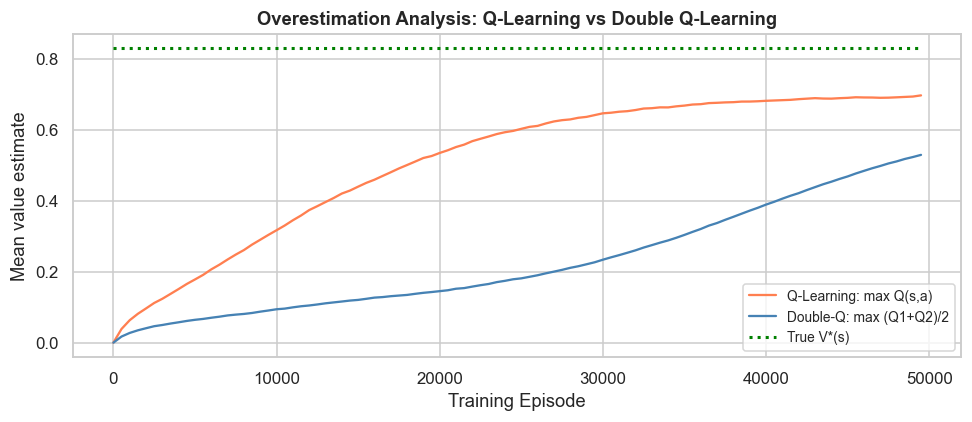
\includegraphics[width=0.85\textwidth]{configA_overestimation.png}
  \caption{Overestimation bias in Config A. Q-Learning Q-values (blue) lie
  systematically above $V^*$ (dashed), computed exactly via value iteration
  on the provided MDP matrices $P$ and $R$. Double Q-Learning (orange) reduces
  the gap, confirming the bias-correction mechanism is active, but the added
  variance from alternating table updates produces a lower test survival rate
  than either Q-Learning or the random baseline.}
  \label{fig:config_a_overestimation}
\end{figure}

\section{Genuine Learning: DQN and PPO Greedy Evaluation}
\label{app:greedy_eval}

\begin{figure}[H]
  \centering
  \begin{minipage}[t]{0.49\textwidth}
    \centering
    \includegraphics[width=\linewidth, height=5cm]{configB_dqn_greedy_eval.png}
  \end{minipage}
  \hfill
  \begin{minipage}[t]{0.49\textwidth}
    \centering
    \includegraphics[width=\linewidth, height=5cm]{configB_ppo_greedy_eval.png}
  \end{minipage}
  \caption{Genuine learning in Config B. \textit{Left}: DQN training return
  (exploration-noisy, grey) versus greedy evaluation at $\varepsilon=0$
  (green), showing ${\approx}11.5$\,pp policy improvement from initialisation.
  \textit{Right}: equivalent view for PPO, showing a slow initial phase while
  advantage estimates accumulate, followed by steeper improvement. Both agents
  learn despite ending below the random baseline.}
  \label{fig:config_b_learning}
\end{figure}

\section{Hyperparameter Tuning Curves}
\label{app:tuning}

\begin{figure}[H]
  \centering
  \begin{minipage}[t]{0.49\textwidth}
    \centering
    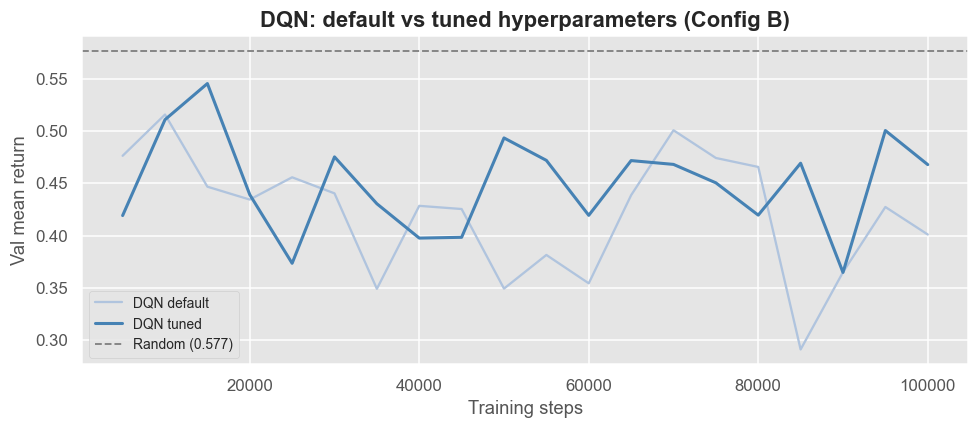
\includegraphics[width=\linewidth, height=5cm]{configB_dqn_tuned_curve.png}
  \end{minipage}
  \hfill
  \begin{minipage}[t]{0.49\textwidth}
    \centering
    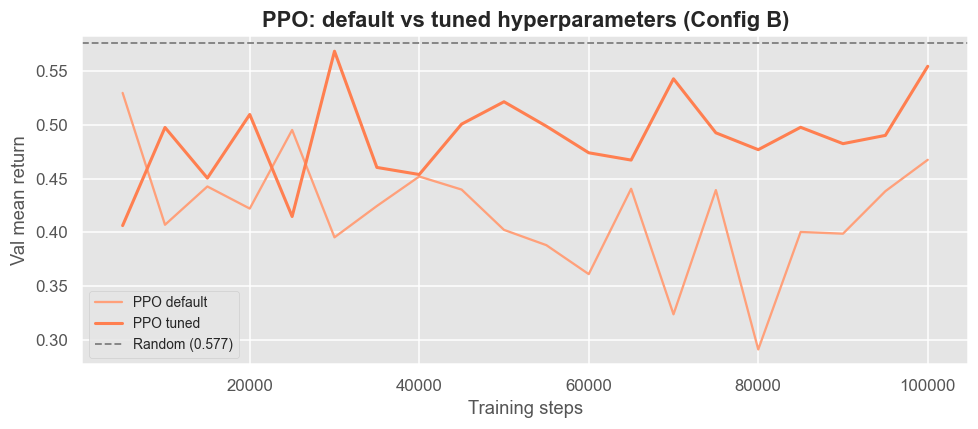
\includegraphics[width=\linewidth, height=5cm]{configB_ppo_tuned_curve.png}
  \end{minipage}
  \caption{Hyperparameter tuning impact for DQN (\textit{left}) and PPO
  (\textit{right}): default versus Optuna-tuned validation curves. Both tuned
  models gain approximately $1$--$2$\,pp, confirming that the binding
  constraint is the sparse reward signal rather than suboptimal hyperparameters.}
  \label{fig:config_b_tuning}
\end{figure}

\section{Hyperparameter Importance (Optuna)}
\label{app:optuna}
% ============================================================

The figures below show the relative importance of each hyperparameter
to final validation performance, estimated by a Random Forest surrogate
fitted to the Optuna trial results. Importance is measured as the
mean decrease in impurity across the surrogate's trees; higher values
indicate that a parameter accounts for more variance in outcome across trials.

\begin{figure}[H]
  \centering
  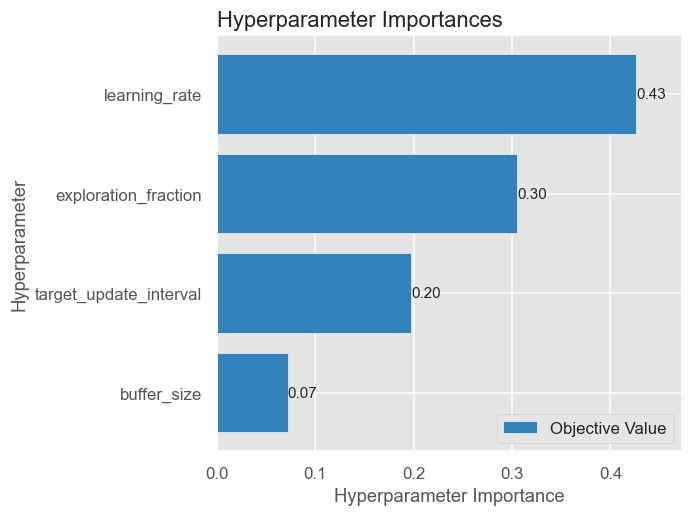
\includegraphics[width=0.85\textwidth]{dqn_optuna_importance.png}
  \caption{DQN hyperparameter importance from Optuna TPE (15 trials,
  30\,000 steps each). Learning rate dominates; target update interval
  and buffer size contribute secondary variance.}
  \label{fig:dqn_optuna}
\end{figure}

\begin{figure}[H]
  \centering
  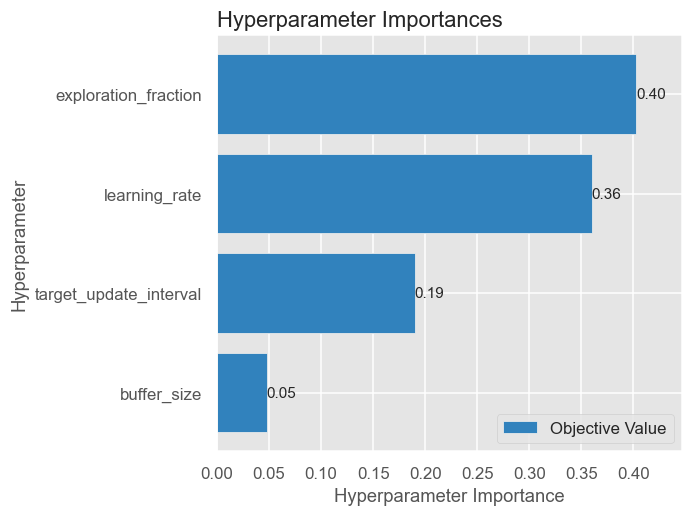
\includegraphics[width=0.85\textwidth]{ppo_optuna_importance.png}
  \caption{PPO hyperparameter importance from Optuna TPE (15 trials,
  30\,000 steps each). Learning rate and rollout length (\texttt{n\_steps})
  account for the majority of outcome variance; entropy coefficient and
  clip range contribute smaller but non-negligible shares.}
  \label{fig:ppo_optuna}
\end{figure}

\end{document}
